%
%  This is part of the SIGI.
%  Copyright (C) 2008 Interlegis
%  See the file relatorio.tex for copying conditions.
%

\section{Organização do sistema}
\label{sec:org}

\subsection{Listagem do conteúdo dos diretórios}
\verbatiminput{../arquivos/tree.txt}

\subsection{Descrição dos arquivos e diretórios}
\begin{description}
\item[COPYING:] Arquivo com a licença do sistema (GPLv3).

\item[LEIA-ME/README:] Contém informações do sistema, nota de
  copyright e instruções de instalação.

\item[devel.db:] Base de dados SQLite utilizada para desenvolvimento
  do sistema.

\item[docs/:] Diretório com toda documentação escrita para o sistema
  (relatórios, manual de instalação, casos de uso, esquema de base de
  dados, etc).

\item[etc/:] Diretório com arquivos variados: configuração do Apache,
  \textit{patchs} de códigos, etc.

\item[media/:] Diretório com arquivos estáticos e de mídia do sistema
  (imagens, CSS, javascripts).

\item[sigi/:] Pacote Python do sistema.

\item[sigi/admin/:] Pacote de código relacionado com a aplicação
  \verb|admin| do Django (\verb|django.contrib.admin|).

\item[sigi/apps/:] Pacote de aplicações do sistema, maiores
  informações na Seção \ref{sec:apps}.

\item[sigi/settings.py:] Configurações padrões do sistema.

\item[sigi/local\_settings.template:] Exemplo de configurações locais
  do sistema (pertinentes à instalação). Deverá ser copiado para
  \verb|sigi/local_settings.py| para sua utilização.

\item[sigi/locale/:] Diretório com localização local do projeto.

\item[sigi/manage.py:] Script de gerenciamento do projeto, gerado pelo
  framework Django.

\item[sigi/templates/:] Diretório com templates HTML do Django.

\item[sigi/urls.py:] Modulo de configuração de URLs.
\end{description}

\subsection{Descrição das aplicações}
\label{sec:apps}
O SIGI é composto de algumas aplicações Django, cada uma com um
propósito bem definido.

Uma aplicação Django é um pacote Python modular, podendo ser
reaproveitado em outros projetos.

Algumas aplicações possuem algum nível de relacionamento com as
outras. A Seção \ref{sec:rel} demonstra o relacionamento entre essas
aplicações.

Segue descrição de cada aplicação:

\begin{description}
\item[sigi.apps.casas:]
  Gerência de Casas Legislativas.

\item[sigi.apps.contatos:]
  Gerência de Contatos do Interlegis com Casas Legislativas,
  fornecedores de equipamentos, serviços e etc.

\item[sigi.apps.convenios:]
  Convênios do Interlegis com as Casas Legislativas.

\item[sigi.apps.inventario:]
  Inventário de equipamentos disponibilizados pelo Interlegis para as
  Casas Legislativas.

\item[sigi.apps.mesas:]
  Composição das Mesas Diretoras das Casas Legislativas.

\item[sigi.apps.parlamentares:]
  Gerência de Parlamentares.

\item[sigi.apps.servicos:]
  Serviços prestados às Casas Legislativas conveniadas ao Interlegis.
\end{description}

\subsubsection{Relacionamento entre as aplicações}
\label{sec:rel}

A Figura \ref{fig:apps} demonstra o relacionamento entre as
aplicações e seus \emph{models}.

Uma seta direcional representa uma relação \textit{muitos para
  um}. Uma seta bidirecional representa uma relação \textit{muitos
  para muitos}.

A seta pontilhada representa uma relação genérica, como descrito na
documentação do Django:\\
http://docs.djangoproject.com/en/dev/ref/contrib/contenttypes/\#id1

\begin{figure}[p]
  \centering
  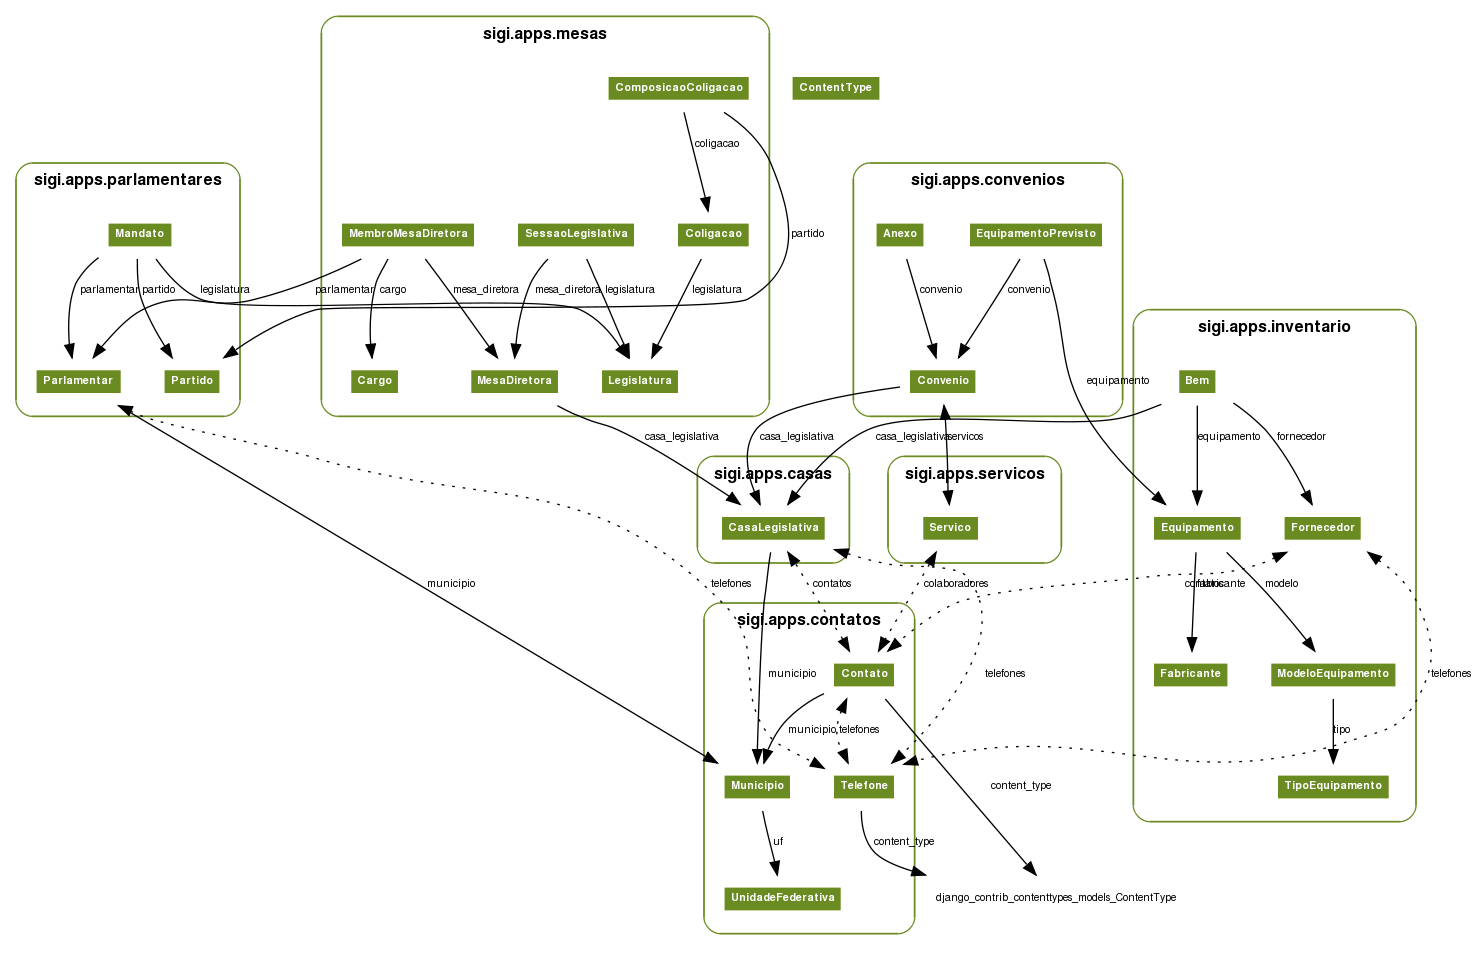
\includegraphics[angle=90,width=130mm]{../imagens/apps.png}
  \caption{Relacionamento entre as aplicações}
  \label{fig:apps}
\end{figure}


%
% Local variables:
%   mode: flyspell
%   TeX-master: "relatorio.tex"
% End:
%
